%%%%%%%%%%%%%%%%%%%%%%%%%%%%%%%%%%%%%
%
%file name = latextop.tex
%
%LATEXTOP TEX%%%%%%%%%%%%%%%%%%%%%%%%%%
%\documentclass[12pt, a4j, landscape]{jarticle}
\documentclass[12pt]{article}
\usepackage{amssymb}
\usepackage[dvips]{epsfig,color}
%\usepackage{reportcover}
%\usepackage{strike}

\setlength{\evensidemargin}{0cm}
\setlength{\oddsidemargin}{0cm}
%\setlength{\textwidth}{26cm}
%\setlength{\textheight}{18cm}
%\setlength{\textwidth}{6.25in}
\setlength{\textwidth}{6.45in}
%\setlength{\textheight}{8.5in}
\setlength{\textheight}{9.2in}
% \setlength{\topmargin}{-1.8cm}
% \setlength{\topmargin}{-1.0cm}
\setlength{\topmargin}{0in}
\setlength{\headheight}{0in}
\setlength{\headsep}{0in}
\setlength{\topskip}{0in} 

\def\@themcountersep{}
\def\thesection{\arabic{section}}
%\def\thesubsection{\thesection\arabic{subsection}}
%\setlength{\evensidemargin}{0in}
%\setlength{\oddsidemargin}{0in}
%\setlength{\textwidth}{6.25in}
%\setlength{\textwidth}{6.45in}
%\setlength{\textheight}{8.5in}
%\setlength{\textheight}{9.2in}
%\setlength{\topmargin}{0in}
%\setlength{\headheight}{0in}
%\setlength{\headsep}{0in}
%\setlength{\itemsep}{-\parsep}
%\renewcommand{\topfraction}{.9}
%\renewcommand{\textfraction}{.1}
\setlength{\parskip}{\medskipamount}

%%%%% Definition of Color ---> %%%%%
\definecolor{TWhite}{rgb}{1,1,1}
\definecolor{TBlack}{rgb}{0,0,0}
\definecolor{TBB}{rgb}{0,0,0.4}
\definecolor{LBlack}{rgb}{0.55,0.52,0.55}
\definecolor{Gray}{rgb}{0.55,0.52,0.55}
% \definecolor{Gray}{rgb}{0,0,0}
% \definecolor{Comment}{rgb}{0.8,0.8,0.8}
\definecolor{Comment}{rgb}{1,1,1}
%\definecolor{TBlue}{rgb}{0,0,0.7}
\definecolor{TBlue}{rgb}{0,0,0.6}
%\definecolor{LBlue}{rgb}{0.35,0.55,0.85}
\definecolor{LBlue}{rgb}{0.30,0.50,0.80}
% \definecolor{LBlue}{rgb}{0,0,0.7}
\definecolor{TGreen}{rgb}{0,0.50,0.10}
\definecolor{LGreen}{rgb}{0.30,0.90,0.30}
\definecolor{Yellow}{rgb}{0.55,0.55,0}
\definecolor{TRed}{rgb}{0.65,0,0}
%\definecolor{LRed}{rgb}{1,0.55,0.55}
%\definecolor{LRed}{rgb}{0.95,0.3,0.2}
\definecolor{LRed}{rgb}{0.95,0.45,0.35}
%\definecolor{TViolet}{rgb}{0.55,0,0.55}
\definecolor{TViolet}{rgb}{0.50,0,0.52}
%\definecolor{LViolet}{rgb}{0.1,0.55,1}
\definecolor{LViolet}{rgb}{0.95,0.55,0.95}
%\definecolor{TBrown}{rgb}{0.5,0.2,0}
\definecolor{TBrown}{rgb}{0.45,0.15,0}
\definecolor{LBrown}{rgb}{0.80,0.50,0}
%%%%%%%%%%
\def\TWhite{\textcolor{TWhite}}
\def\TBlack{\textcolor{TBlack}}
\def\TBB{\textcolor{TBB}}
\def\LBlack{\textcolor{LBlack}}
\def\Gray{\textcolor{Gray}}
\def\TBlue{\textcolor{TBlue}}
% \def\TBlue{\TBlack}
\def\LBlue{\textcolor{LBlue}}
\def\TGreen{\textcolor{TGreen}}
% \def\TGreen{\TBlack}
\def\LGreen{\textcolor{LGreen}}
\def\Yellow{\textcolor{Yellow}}
\def\TRed{\textcolor{TRed}}
% \def\TRed{\TBlack}
\def\LRed{\textcolor{LRed}}
\def\TOrange{\textcolor{LRed}}
\def\TViolet{\textcolor{TViolet}}
% \def\TViolet{\Black}
\def\LViolet{\textcolor{LViolet}}
\def\TBrown{\textcolor{TBrown}}
\def\LBrown{\textcolor{LBrown}}
%%%%% <--- Definition of Color%%%%%

%\include{abbrev}
\catcode`@=11
\renewcommand{\@begintheorem}[2]{\it \trivlist
       \item[\hskip \labelsep{\bf #1\ #2{.}}]}
\renewcommand{\@opargbegintheorem}[3]{\it \trivlist
       \item[\hskip \labelsep{\bf #1\ #2\ (#3) {:}}]}
\catcode`@=12
%\newenvironment{PROOF}
%  {\hangindent=10pt \hangafter=0  \hskip 3 pt {\it Proof:\hskip 3pt}}
%  {\hskip 3pt \vrule height4pt width3pt depth2pt
%                \par\vskip 3pt plus 6pt}
  \newcommand{\proof}[1]{\hangindent=10pt \hangafter=0  \hskip 3 pt
                {\it Proof:\hskip 3pt} #1
               \hskip 3 pt \vrule height4pt  width3pt depth2pt
               \par\vskip 3pt plus 6pt
             }
  \newcommand{\proofof}[2]{\hangindent=10pt \hangafter=0  \hskip 3 pt
                {\bf Proof of #1:\hskip 3pt} #2
               \hskip 3 pt \vrule height4pt  width3pt depth2pt
               \par\vskip 3pt plus 6pt
             }

%\newtheorem{FIGURE}{figure}[section]
%\newcommand{\fig}{\begin{FIGURE}}
%\newcommand{\efig}{\end{FIGURE}}
\newtheorem{THEO}{Theorem}[section]
\newtheorem{ALGo}[THEO]{Algorithm}
\newtheorem{CONJ}[THEO]{Conjecture}
\newtheorem{COND}[THEO]{Condition}
\newtheorem{CORO}[THEO]{Corollary}
\newtheorem{DEFI}[THEO]{Definition}
\newtheorem{EXAMP}[THEO]{Example}
\newtheorem{FACT}[THEO]{Fact}
\newtheorem{HYPO}[THEO]{Hypothesis}
\newtheorem{LEMM}[THEO]{Lemma}
\newtheorem{PROB}[THEO]{Problem}
\newtheorem{PROP}[THEO]{Proposition}
\newtheorem{REMA}[THEO]{Remark}
\newcommand{\theo}{\begin{THEO}}
\newcommand{\algo}{\begin{ALGo} \rm}
\newcommand{\cond}{\begin{COND}}
\newcommand{\conj}{\begin{CONJ}}
\newcommand{\coro}{\begin{CORO}}
\newcommand{\defi}{\begin{DEFI} \rm}
\newcommand{\examp}{\begin{EXAMP} \rm}
\newcommand{\fact}{\begin{FACT}}
\newcommand{\hypo}{\begin{HYPO} \rm}
\newcommand{\lemm}{\begin{LEMM}}
\newcommand{\prob}{\begin{PROB} \rm}
\newcommand{\prop}{\begin{PROP}}
\newcommand{\rema}{\begin{REMA} \rm}
\newcommand{\etheo}{\end{THEO}}
\newcommand{\ealgo}{\end{ALGo}}
\newcommand{\econd}{\end{COND}}
\newcommand{\econj}{\end{CONJ}}
\newcommand{\ecoro}{\end{CORO}}
\newcommand{\edefi}{\end{DEFI}}
\newcommand{\eexamp}{\end{EXAMP}}
\newcommand{\efact}{\end{FACT}}
\newcommand{\ehypo}{\end{HYPO}}
\newcommand{\elemm}{\end{LEMM}}
\newcommand{\eprob}{\end{PROB}}
\newcommand{\eprop}{\end{PROP}}
\newcommand{\erema}{\end{REMA}}
\def\br{\hfill\break}
\def\mAth{\mathsurround=0pt}
\def\eqalign#1{\,\vcenter{\openup1\jot \mAth
   \ialign{\strut\hfil$\displaystyle{##}$&$\displaystyle{{}##}$\hfil
     \crcr#1\crcr}}\,}

%
%file name = bflatex.tex
%
\def\0{\mbox{\bf 0}}
\def\1{\mbox{\bf 1}}
\def\2{\mbox{\bf 2}}
\def\3{\mbox{\bf 3}}
\def\4{\mbox{\bf 4}}
\def\5{\mbox{\bf 5}}
\def\6{\mbox{\bf 6}}
\def\7{\mbox{\bf 7}}
\def\8{\mbox{\bf 8}}
\def\9{\mbox{\bf 9}}
\def\a{\mbox{\boldmath $a$}}
\def\b{\mbox{\boldmath $b$}}
%\def\c{\mbox{\boldmath $c$}}
\def\cc{\mbox{\boldmath $c$}}
\def\d{\mbox{\boldmath $d$}}
\def\e{\mbox{\boldmath $e$}}
\def\f{\mbox{\boldmath $f$}}
\def\g{\mbox{\boldmath $g$}}
\def\h{\mbox{\boldmath $h$}}
\def\i{\mbox{\boldmath $i$}}
\def\j{\mbox{\boldmath $j$}}
\def\k{\mbox{\boldmath $k$}}
\def\l{\mbox{\boldmath $l$}}
\def\m{\mbox{\boldmath $m$}}
\def\n{\mbox{\boldmath $n$}}
\def\o{\mbox{\boldmath $o$}}
\def\p{\mbox{\boldmath $p$}}
\def\q{\mbox{\boldmath $q$}}
\def\r{\mbox{\boldmath $r$}}
\def\s{\mbox{\boldmath $s$}}
\def\t{\mbox{\boldmath $t$}}
\def\u{\mbox{\boldmath $u$}}
\def\v{\mbox{\boldmath $v$}}
\def\w{\mbox{\boldmath $w$}}
\def\x{\mbox{\boldmath $x$}}
\def\y{\mbox{\boldmath $y$}}
\def\z{\mbox{\boldmath $z$}}
\def\A{\mbox{\boldmath $A$}}
\def\B{\mbox{\boldmath $B$}}
\def\C{\mbox{\boldmath $C$}}
\def\D{\mbox{\boldmath $D$}}
\def\E{\mbox{\boldmath $E$}}
\def\F{\mbox{\boldmath $F$}}
\def\G{\mbox{\boldmath $G$}}
\def\H{\mbox{\boldmath $H$}}
\def\I{\mbox{\boldmath $I$}}
\def\J{\mbox{\boldmath $J$}}
\def\K{\mbox{\boldmath $K$}}
\def\L{\mbox{\boldmath $L$}}
\def\M{\mbox{\boldmath $M$}}
\def\N{\mbox{\boldmath $N$}}
\def\O{\mbox{\boldmath $O$}}
\def\P{\mbox{\boldmath $P$}}
\def\Q{\mbox{\boldmath $Q$}}
\def\R{\mbox{\boldmath $R$}}
\def\S{\mbox{\boldmath $S$}}
\def\T{\mbox{\boldmath $T$}}
\def\U{\mbox{\boldmath $U$}}
\def\V{\mbox{\boldmath $V$}}
\def\W{\mbox{\boldmath $W$}}
\def\X{\mbox{\boldmath $X$}}
\def\Y{\mbox{\boldmath $Y$}}
\def\Z{\mbox{\boldmath $Z$}}
\def\AC{\mbox{$\cal A$}}
\def\BC{\mbox{$\cal B$}}
\def\CC{\mbox{$\cal C$}}
\def\DC{\mbox{$\cal D$}}
\def\EC{\mbox{$\cal E$}}
\def\FC{\mbox{$\cal F$}}
\def\GC{\mbox{$\cal G$}}
\def\HC{\mbox{$\cal H$}}
\def\IC{\mbox{$\cal I$}}
\def\JC{\mbox{$\cal J$}}
\def\KC{\mbox{$\cal K$}}
\def\LC{\mbox{$\cal L$}}
\def\MC{\mbox{$\cal M$}}
\def\NC{\mbox{$\cal N$}}
\def\OC{\mbox{$\cal O$}}
\def\PC{\mbox{$\cal P$}}
\def\QC{\mbox{$\cal Q$}}
\def\RC{\mbox{$\cal R$}}
\def\SC{\mbox{$\cal S$}}
\def\TC{\mbox{$\cal T$}}
\def\UC{\mbox{$\cal U$}}
\def\VC{\mbox{$\cal V$}}
\def\WC{\mbox{$\cal W$}}
\def\XC{\mbox{$\cal X$}}
\def\YC{\mbox{$\cal Y$}}
\def\ZC{\mbox{$\cal Z$}}
\def\ACs{\mbox{\tiny $\cal A$}}
\def\BCs{\mbox{\tiny $\cal B$}}
\def\CCs{\mbox{\tiny $\cal C$}}
\def\DCs{\mbox{\tiny $\cal D$}}
\def\ECs{\mbox{\tiny $\cal E$}}
\def\FCs{\mbox{\tiny $\cal F$}}
\def\GCs{\mbox{\tiny $\cal G$}}
\def\HCs{\mbox{\tiny $\cal H$}}
\def\ICs{\mbox{\tiny $\cal I$}}
\def\JCs{\mbox{\tiny $\cal J$}}
\def\KCs{\mbox{\tiny $\cal K$}}
\def\LCs{\mbox{\tiny $\cal L$}}
\def\MCs{\mbox{\tiny $\cal M$}}
\def\NCs{\mbox{\tiny $\cal N$}}
\def\OCs{\mbox{\tiny $\cal O$}}
\def\PCs{\mbox{\tiny $\cal P$}}
\def\QCs{\mbox{\tiny $\cal Q$}}
\def\RCs{\mbox{\tiny $\cal R$}}
\def\SCs{\mbox{\tiny $\cal S$}}
\def\TCs{\mbox{\tiny $\cal T$}}
\def\UCs{\mbox{\tiny $\cal U$}}
\def\VCs{\mbox{\tiny $\cal V$}}
\def\WCs{\mbox{\tiny $\cal W$}}
\def\XCs{\mbox{\tiny $\cal X$}}
\def\YCs{\mbox{\tiny $\cal Y$}}
\def\ZCs{\mbox{\tiny $\cal Z$}}

\def\Real{\mbox{$\mathbb{R}$}}
\def\Integer{\mbox{$\mathbb{Z}$}}
\def\balpha{\mbox{\boldmath $\alpha$}}
\def\bbeta{\mbox{\boldmath $\beta$}}
\def\bgamma{\mbox{\boldmath $\gamma$}}

\def\bdelta{\mbox{\boldmath $\delta$}}

\def\bepsilon{\mbox{\boldmath $\epsilon$}}

\def\salpha{\mbox{\scriptsize \boldmath $\alpha$}}
\def\sbeta{\mbox{\scriptsize \boldmath $\beta$}}
\def\sgamma{\mbox{\scriptsize \boldmath $\gamma$}}
\def\s0{\mbox{\scriptsize \boldmath $0$}}

\def\sdelta{\mbox{\scriptsize \boldmath $\delta$}}

\def\sepsilon{\mbox{\scriptsize \boldmath $\epsilon$}}


\def\blambda{\mbox{\boldmath $\lambda$}}
\def\bLambda{\mbox{\boldmath $\Lambda$}}
\def\hLambda{\mbox{$\widehat{\bLambda}$}}
\def\bmu{\mbox{\boldmath $\mu$}}
\def\bvarphi{\mbox{\boldmath $\varphi$}}
\def\bpsi{\mbox{\boldmath $\psi$}}
\def\FCB{\mbox{\boldmath $\cal F$}}
\def\barSigma{\mbox{$\overline{\Sigma}$}}
\def\barAC{\mbox{$\overline{\AC}$}}
\def\tAC{\mbox{$\widetilde{\AC}$}}
\def\tBC{\mbox{$\widetilde{\BC}$}}
\def\tG{\mbox{$\widetilde{\G}$}}
\def\tGC{\mbox{$\widetilde{\GC}$}}
\def\sGC{\mbox{\scriptsize ${\GC}$}}
\def\hGC{\mbox{$\widehat{\GC}$}}
\def\tV{\mbox{$\widetilde{V}$}}
\def\hV{\mbox{$\widehat{V}$}}
\def\tbV{\mbox{$\widetilde{\V}$}}
\def\hbV{\mbox{$\widehat{\V}$}}
\def\tw{\mbox{$\widetilde{w}$}}
\def\hw{\mbox{$\widehat{w}$}}
\def\bbW{\mbox{$\overline{\W}$}}
\def\boldSigma{\mbox{\boldmath $\Sigma$}}
\def\boldXi{\mbox{\boldmath $\Xi$}}


% \def\IM{\mbox{$\I \hspace{-0.6mm}$mat}}
\def\IM{\mbox{$\A$}}
\def\barIM{\mbox{$\overline{\A}$}}
\def\barG{\mbox{$\overline{G}$}}
\def\barE{\mbox{$\overline{E}$}}


\begin{document}



\thispagestyle{empty}

\noindent
\parbox[t]{14cm}
{User Manual for {\bf SFSDP}:  a {\bf S}parse  Version of  {\bf F}ull   {\bf S}emi{\bf D}efinite
	{\bf P}rogramming Relaxation  for Sensor Network Localization Problems} \\~\vspace{0.2cm}\\
$\mbox{Sunyoung Kim}^{\star}$,
$\mbox{Masakazu Kojima}^{\dagger}$, 
$\mbox{Hayato Waki}^{\ddagger}$, and 
$\mbox{Makoto Yamashita}^{\sharp}$\vspace{0.2cm}\\
August 2008, Revised January 2010

\medskip

\noindent
{\bf Abstract.} \vspace{2mm}\\ 
{\bf SFSDP} is a Matlab package for solving 
sensor network localization problems. 
The package contains  four functions, SFSDP.m, SFSDPplus.m, generateProblem.m, test\_SFSDP.m, 
and  some numerical examples. 
The function SFSDP.m is a Matlab implementation of the semidefinite programming 
(SDP) relaxation  proposed in the recent paper by Kim, Kojima and Waki 
for sensor network localization problems, 
as a sparse version of the full semidefinite programming relaxation (FSDP)  
by Biswas and Ye. To improve the efficiency of FSDP, SFSDP.m  exploits 
the aggregated and correlative sparsity of a sensor network localization problem. 
The function SFSDPplus.m analyzes the input data of a sensor network localization problem, 
solves the problem, and displays graphically computed locations of sensors. The function generateProblem.m
creates numerical examples of sensor network localization problems with representative
anchor locations. The function test\_SFSDP.m is for numerical experiments using SFSDPplus.m 
with test problems  generated by generateProblem.m. 
The  package {\bf SFSDP} and this manual
are available at

\vspace{-3mm} 

\begin{center}
\mbox{http://www.is.titech.ac.jp/$\sim$kojima/SFSDP}
\end{center}

\medskip
  
\noindent
{\bf Key words. } \vspace{0.1cm} \\
Sensor network localization problems, 
Semidefinite programming relaxation, Sparsity exploitation,  Matlab software package.

\vspace{0.5cm}

\noindent
\parbox[t]{0.5cm}{$\star$}
\parbox[t]{14.9cm}{Department of Mathematics, Ewha W. University,
11-1 Dahyun-dong, Sudaemoon-gu, Seoul 120-750 Korea.
 S. Kim's research was supported
by KOSEF 2009-007-1314.
{\it skim@ewha.ac.kr}
}

\medskip

\noindent
\parbox[t]{0.5cm}{$\dagger$}
\parbox[t]{14.9cm}{Department of Mathematical and Computing Sciences,
                      Tokyo Institute of Technology,
                      2-12-1 Oh-Okayama, Meguro-ku, Tokyo 152-8552 Japan.
                      M. Kojima's research was supported by Grant-in-Aid for
                                         Scientific Research (B) 19310096.
{\it kojima@is.titech.ac.jp}
}


\medskip

\noindent
\parbox[t]{0.5cm}{$\ddagger$}
\parbox[t]{14.9cm}{
Department of Computer Science,
    The University of Electro-Communications \\
        1-5-1 Chofugaoka, Chofu-shi, Tokyo, Japan. H. Waki's research was supported by
Grant-in-Aid for JSPS Fellows 20003236.  {\it
hayato.waki@jsb.cs.uec.ac.jp}
}

\medskip

\noindent
\parbox[t]{0.5cm}{$\sharp$}
\parbox[t]{14.9cm}{Department of Mathematical and Computing Sciences,
                      Tokyo Institute of Technology,
                      2-12-1 Oh-Okayama, Meguro-ku, Tokyo 152-8552 Japan.
                      M. Yamashita's research was supported by Grant-in-Aid for
                                        Young Scientists  (B) 21710148.
{\it Makoto.Yamashita@is.titech.ac.jp}
}


\newpage



\section{Introduction}


For a  network of $n$ sensors,  where $n >  m$,
a sensor network localization problem is to locate $m$ sensors that fit the given distances 
if a subset of distances and some sensors of known position (called anchors)
are provided. 
Various approaches 
\cite{ALFAKIH99,DOHERTY01,EREN04,GANESAN02,HOWARD01,TSENG07}
 have been proposed for the problem 
to approximate the solutions.  Full semidefinite programming relaxation (FSDP) 
 was introduced by Biswas and Ye in \cite{BISWAS04}, 
and  a number of solution methods based on SDP relaxation have followed
\cite{BISWAS06a,BISWAS06b,BISWAS06c,NIE06,WANG07}. 

We introduce a Matlab package SFSDP  for 
solving sensor network localization problems by 
SDP relaxation.
The main function SFSDP.m of the package is an implementation of the SDP relaxation 
proposed in the recent paper by Kim, Kojima and Waki \cite{KIM08}.  
SFSDP.m is intended to improve the efficiency of Biswas and Ye's FSDP \cite{BISWAS04}
by exploiting the sparsity, the aggregated and correlative sparsity 
\cite{FUKUDA00,NAKATA03,KOBAYASHI07a},  of sensor network problems. 
The quality of obtained solution by SFSDP.m remains equivalent to that by FSDP.
As a result,  SFSDP.m can handle larger-sized  sensor network problems, e.g.,
up to 6000 sensors in 2-dimensional case, than FSDP. 

SFSDP.m can solve the problem with exact  and noisy distances.
To describe a form of the sensor network localization problem that can be  solved by
SFSDP.m,  we consider  a problem with $m$ sensors and $m_a$ $(=n-m)$ anchors. 
Let $\rho > 0$ be a radio range,  which determines the set $\NC^{\rho}_x$ of pairs of 
sensors $p$ and $q$ such that their unknown (Euclidean) distance $d_{pq}$ is not greater than $\rho$, 
and the set $\NC^{\rho}_a$ of pairs of a sensor $p$ and an anchor $r$ 
such that their distance $d_{pr}$ does not exceed $\rho$;  
\begin{eqnarray}
\left. 
\begin{array}{lcl} 
\NC^{\rho}_x & = & \{ (p,q) : 1 \leq p < q \leq m, \| \bar{\x}_p - \bar{\x}_q \| \leq \rho \}, \\ 
\NC^{\rho}_a & = & \{ (p,r) : 1 \leq p \leq m,  m+1 \leq r \leq n, \| \bar{\x}_p - \a_r \| \leq \rho \},
\end{array}
\right\} 
\label{radiorange}
\end{eqnarray}
where $\bar{\x}_p$ denotes unknown location of sensor $p$ and $\a_r$ known location of 
anchor $r$. Let $\NC_x$ be a subset of $\NC^{\rho}_x$ and 
and $\NC_a$ a subset of $\NC^{\rho}_a$. 
 For $\ell$-dimensional problem,  an $\ell \times m$ matrix variable 
$\X = (\x_1,\ldots,\x_m) \in \Real^{\ell \times m}$  denotes location of the sensors. 
SFSDP.m can solve the problem of $\ell = 2 $ or $3$.
By introducing zero objective function and
 the distance equations  as constraints, we have the following form of the sensor network
 localization problem with exact distances.  
\begin{equation}
\left.
\begin{array}{lll}
\mbox{minimize }  & 0 \\
\mbox{subject to } &
\displaystyle  d_{pq}^2   
= \|\x_p - \x_q\| ^2 \ \  (p,q) \in \NC_x, \\
& \displaystyle  d_{pr}^2  
=  \|\x_p - \a_r\| ^2 \ \  (p,r) \in \NC_a. 
\end{array}
 \right\}
 \label{POPnoNoise}
\end{equation}

When the distance involves noise, the following problem is considered. 
\begin{equation} 
\left.
\begin{array}{ll}
\mbox{minimize }  & 
\displaystyle \sum_{(p,q) \in \NC_x} \left( \epsilon_{pq}^+ + \epsilon_{pq}^- \right) 
  + \sum_{(p,r) \in \NC_a} \left( \epsilon_{pr}^+  + \epsilon_{pr}^- \right) \\ 
\mbox{subject to } & 
\displaystyle  \hat{d}_{pq}^2  = 
\|\x_p - \x_q\| ^2 
+ \epsilon_{pq}^+ - \epsilon_{pq}^-  \ \  
 (p,q) \in \NC_x, \\
& \displaystyle  \hat{d}_{pr}^2 = 
 \|\x_p - \a_r\| ^2 
 + \epsilon_{pr}^+ - \epsilon_{pr}^- \  \   (p,r) \in \NC_a, \\
&\displaystyle  \epsilon_{pq}^+ \geq 0, \ \epsilon_{pq}^- \geq 0, \ (p,q) \in \NC_x, \\
& \displaystyle  \epsilon_{pr}^+ \geq 0, \ \epsilon_{pr}^- \geq 0,
(p,r) \in \NC_a.
\end{array}
\right\}
\label{POPnoise}
\end{equation} 
Here $\epsilon_{pq}^+ + \epsilon_{pq}^-$  \ (or $\epsilon_{pr}^+ + \epsilon_{pr}^-$) indicates 
 1-norm error in the estimated distance $\hat{d}_{pq}$ between
sensors $p$ and $q$ (or an estimated distance $\hat{d}_{pr}$ between
sensor $p$ and anchor $r$, respectively). 


When a sensor network problem of the form (\ref{POPnoNoise}) or (\ref{POPnoise})
has many  equality constraints that may be redundant,   
the resulting SDP relaxation problem can be too large to solve. 
To deal with such a problem, SFSDP.m replaces $\NC_x$ and $\NC_a$
by smaller subsets of them,  $\NC'_x$ and $\NC'_a$, respectively, before applying the sparse SDP 
relaxation to the problem (\ref{POPnoNoise}) or (\ref{POPnoise}). Then,
 the resulting SDP relaxation problem becomes smaller and sparser. 
This process  is a key for solving  large scale sensor network localization problems 
efficiently by SFSDP.m.  See Section 4.1 of \cite{KIM08} for 
more details. 
We assume that either 
(i) (noisy) distance information is available between a fairly large number of sensors and anchors 
in the original problem  (\ref{POPnoNoise}) or (\ref{POPnoise}) 
to extract a smaller-sized subproblem satisfying the sparsity (the aggregated and 
correlative sparsity) or (ii) the original problem itself is sparse.  If we take 
$\NC^{\rho}_x$ and $\NC^{\rho}_a$ (or their subsets large enough) for $\NC_x$ and $\NC_a$, 
respectively,  the assumption (i) is usually satisfied. We should note, however, that
 SFSDP.m may fail to solve the problem efficiently if neither (i) nor (ii) is satisfied. 


Edge-based SDP (ESDP) and node-based SDP (NSDP) relaxations were introduced in \cite{WANG07}
to improve the computational efficiency of the original Biswas-Ye SDP relaxation 
FSDP. These  SDP relaxations
are further relaxations of FSDP, hence, they are theoretically
weaker than FSDP. SFSDP.m, however,  is shown to be equivalent
to FSDP in \cite{KIM08}.

\begin{figure}
\label{structure}
\begin{center}
\hspace*{-3cm}
\epsfig{file=sFSDP.eps,height=11cm}
\vspace*{-3cm}
\caption{The structure of SFSDP}
\label{STRUCTURE}
\end{center}
\end{figure}


The structure of the  package SFSDP is shown in Figure \ref{STRUCTURE}. 
In addition to SFSDP.m, the package includes three functions, SFDPplus.m, generateProblem.m, 
and test\_SFDP.m. 
The function SFDPplus.m is designed for users who want to solve their own sensor network localization 
problems.  Users can use SFSDP.m via SFSDPplus.m or SFSDP.m directly.  
After analyzing input data of a given problem, SFSDPplus.m  solves the problem by SFSDP.m, and 
displays graphically  computed locations of sensors.  Users can call either of 
SFSDP.m and SFDPplus.m from their own Matlab function that can provide necessary input 
data.  SFSDP.m calls SDPA \cite{FUJISAWA08}, available 
at \cite{SDPA}, or SeDuMi \cite{STURM99}, available at \cite{SEDUMI}, 
 to solve SDP relaxation problems.  
 For larger problems, using SDPA requires much less computational time. See Appendix. 

The other two functions 
generateProblem.m and test\_SFDP.m are for users interested in numerical 
experiments using SFDPplus.m.  The function generateProblem.m 
creates numerical examples of sensor network localization problems with representative
anchor locations. The function test\_SFSDP.m is for numerical experiments on SFSDPplus.m 
applied to test problems  generated by generateProblem.m. 
We discuss in detail input and output for the functions 
SFSDP.m,  SFSDPplus.m, generateProblem.m and test\_SFSDP.m  in Section \ref{IOP}.

\section{Sample Run Using SDPA}
\label{EXEC}

The usage of SFSDPplus.m, SFSDP.m, generateProblems.m, and test\_SFSDP.m is described 
in this section.

\subsection{SFSDPplus.m}
\label{SFSDPplus}

We show how SFSDPplus.m can be executed with an illustrative example.
A small problem of $3$ sensors and $4$ anchors
in the two dimensional space
is generated with the following xMatrix0 and distanceMatrix0. 
Assume that the sensors are located at $(0.3, 0.4)$, $(0.3, 0.6)$, and $(0.7, 0.6)$
and the anchors are at $(0, 0), (0,1), (1, 0), $ and $(1,1)$. Then,
we prepare input data and parameters as follows:
\begin{verbatim}
>> sDim= 2; noOfSensors= 3; noOfAnchors= 4;
>> pars.free= 0; pars.eps= 1.0000e-05; pars.minDegree= 4; pars.objSW = 1;
>> pars.noisyFac= 0; 
\end{verbatim} 
The size of 
xMatrix0 is 
$\mbox{sDim} \times \mbox{(noOfSensors + noOfAnchors)}$ matrix
and its elements  are:
\begin{verbatim}
>> xMatrix0
xMatrix0 =
    0.3000    0.3000    0.7000         0         0    1.0000    1.0000
    0.4000    0.6000    0.6000         0    1.0000         0    1.0000
\end{verbatim} 
The first three columns of xMatrix0, which indicate the
 true location of sensors, can be omitted
 for general cases where  the locations of sensors are unknown.

The distance information is stored in a 
matrix called distanceMatrix0.
The size of distanacneMatrix0 is $\mbox{noOfSensors} \times \mbox{(noOfSensors +
noOfAnchors)}$,  and 
the $(p,q)$th component of
distanceMatrix0  indicates the distance between sensors $p$ and $q$, or equivalently, between
xMatrix0(:,$p$) and xMatrix0(:,$q$).  Note that distanceMatrix0 is upper triangular; 
distanceMatrix0$(p,q) = 0$ if $p \geq q$.
\begin{verbatim}    
>> distanceMatrix0
distanceMatrix0 =
  0   0.219579   0.414739   0.501646   0.756645           0          0
  0          0   0.356155   0.629003   0.471282           0          0
  0          0          0          0          0    0.647147   0.468894
\end{verbatim}    
 Then, issue a command: 
 \begin{verbatim}
>>[xMatrix,distanceMatrix,info,pars] = SFSDPplus(sDim,noOfSensors,...
                  noOfAnchors,xMatrix0,distanceMatrix0,pars);
\end{verbatim}    
Then, the following is displayed on the screen.
\begin{verbatim}
## sDim = 2, noOfSensors = 3, noOfAnchors = 4
## the number of dist. eq. between two sensors  = 3
## the number of dist. eq. between a sensor & an anchor = 6
## the min., max. and ave. degrees over sensor nodes = 4, 4,   4.00
## +0.0000e+00 <= x(1) <= +1.0000e+00
## +0.0000e+00 <= x(2) <= +1.0000e+00
## the max. radio range = 6.7082e-01, the estimated noisy factor = 8.3330e-02

SFSDP --- A Sparse version of FSDP (Biswas and Ye)
Sunyoung Kim, Masakazu Kojima, Hayato Waki and Makoto Yamashita
Version 1.22, January 2010

## sDim = 2, noOfSensors = 3, noOfAnchors = 4
## pars: SDPsolver = sdpa, eps = 1.00e-07
## pars: sparseSW = 1, minDegree = 4, edgeSelectionSW = 1
## pars: objSW = 1, noisyFac = 8.3e-02, regTermFactor = 0.00
## the number of dist. eq. used in SFSDP between two sensors  = 3
## the number of dist. eq. used in SFSDP between a sensor & an anchor = 6
## the min., max. and ave. degrees over sensor nodes = 4, 4,   4.00
## elapsed time for generating an SDP relaxation problem =     0.09
-SeDuMi Wrapper for SDPA Start-
Note: pars information [4th argument] is not used
Free Variables are divided into positive and negative part of LP cone
Converted to SDPA internal data / Starting SDPA main loop
Converting optimal solution to Sedumi format
-SeDuMi Wrapper for SDPA End-
## elapsed time for retrieving an optimal solution =     0.01
## elapsed time for SDP solver =     0.07
## mean error in dist. eq. = 1.34e-02, max. error in dist. eq. = 7.29e-02
## rmsd = 6.21e-02
## see Figure 101
## elapsed time for a gradient method =     0.06
## mean error in dist. eq. = 1.57e-02, max. error in dist. eq. = 4.56e-02
## rmsd = 4.67e-02
## see Figure 103
\end{verbatim}

\begin{figure}
\epsfig{file=example2LocationSDP.eps,scale=0.43}  \hspace{1mm}
\epsfig{file=example2LocationGrad.eps,scale=0.43}
\caption{An example with three sensors and four anchors. 
Before and after the refinement using the gradient method.}
\label{EG0}
\end{figure}

Figure \ref{EG0} is displayed  at the end of execution. In Figure \ref{EG0} and throughout,
a circle indicates the true location of a sensor, $\star$ the computed location of a sensor,
and a line segment a difference between  the true  and computed location.
The input data and parameters of this  example are stored in the file examples/example1.mat 
of the package, and can be loaded by
\begin{verbatim}
>> load example1.mat
\end{verbatim}
instead of specifying them from the command window. 

Next, we consider a 2-dimensional  problem with 500 sensors and 100 anchors placed 
randomly in the region $[0,1] \times [0,1]$ and noisy distances.  As in practical applications, we assume that
the locations of the sensors are not known.  For instance, suppose that 
xMatrix0 includes only 100 locations of anchors. To solve the 
problem, the following command can be used after loading the data stored in the file
d2n01s500a100ns.mat, which is included in the directory examples of the package. 
\begin{verbatim}
>> load d2n01s500a100ns.mat;
>>[xMatrix,distanceMatrix,info,pars] = SFSDPplus(sDim,noOfSensors,...
                  noOfAnchors,xMatrix0,distanceMatrix0,pars);
## only anchor locations are given
## sDim = 2, noOfSensors = 500, noOfAnchors = 100
## the number of dist. eq. between two sensors  = 8171
## the number of dist. eq. between a sensor & an anchor = 3000
## the min., max. and ave. degrees over sensor nodes = 24, 167,  38.68
## no location for sensors is given

SFSDP --- A Sparse version of FSDP (Biswas and Ye)
Sunyoung Kim, Masakazu Kojima, Hayato Waki and Makoto Yamashita
Version 1.22, January 2010

## sDim = 2, noOfSensors = 500, noOfAnchors = 100
## pars: SDPsolver = sdpa, eps = 1.00e-05
## pars: sparseSW = 1, minDegree = 4, edgeSelectionSW = 1
## pars: objSW = 1, noisyFac = 1.0e-01, regTermFactor = 0.00
## the number of dist. eq. used in SFSDP between two sensors  = 976
## the number of dist. eq. used in SFSDP between a sensor & an anchor = 3000
## the min., max. and ave. degrees over sensor nodes = 8, 112,   9.90
## elapsed time for generating an SDP relaxation problem =     0.52
-SeDuMi Wrapper for SDPA Start-
Note: pars information [4th argument] is not used
Free Variables are divided into positive and negative part of LP cone
Converted to SDPA internal data / Starting SDPA main loop
Converting optimal solution to Sedumi format
-SeDuMi Wrapper for SDPA End-
## elapsed time for retrieving an optimal solution =     0.07
## elapsed time for SDP solver =     1.66
## mean error in dist. eq. = 2.93e-04, max. error in dist. eq. = 9.63e-02
## see Figure 101
## elapsed time for a gradient method =     0.71
## mean error in dist. eq. = 1.99e-04, max. error in dist. eq. = 6.36e-02
## see Figure 103
\end{verbatim}
Figure \ref{EG1NS} is displayed at the end of execution.
\begin{figure}
\epsfig{file=eg1beRefineNS.eps,scale=0.43}  \hspace{1mm}
\epsfig{file=eg1afRefineNS.eps,scale=0.43}
\caption{A 2-dimensional  problem with 500 sensors  (no information on their location) and 100 anchors and noisy distance. 
Before and after the refinement using the gradient method.}
\label{EG1NS}
\end{figure}
After obtaining a solution with SFSDP.m, SFSDPplus.m refines the solution using 
the function refineposition.m, 
which is a Matlab implementation of the gradient method provided by Prof. Kim-Chuan Toh.
The figure on the right of Figure \ref{EG1NS} is attained after applying the function. 

We solve the same problem with information on the location of sensors to see how accurately 
the computed locations of sensors approximates the true locations of
sensors. 
Note that we load d2n01s500a100.mat instead of
d2n01s500a100ns.mat. 
\begin{verbatim}
>> load d2n01s500a100.mat;
>>[xMatrix,distanceMatrix,info,pars] = SFSDPplus(sDim,noOfSensors,...
                  noOfAnchors,xMatrix0,distanceMatrix0,pars);
## sDim = 2, noOfSensors = 500, noOfAnchors = 100
## the number of dist. eq. between two sensors  = 8171
## the number of dist. eq. between a sensor & an anchor = 3000
## the min., max. and ave. degrees over sensor nodes = 24, 167,  38.68
## +1.5003e-03 <= x(1) <= +9.9912e-01
## +9.7480e-04 <= x(2) <= +9.9948e-01
## the max. radio range = 3.0000e-01, the estimated noisy factor = 9.9337e-02

SFSDP --- A Sparse version of FSDP (Biswas and Ye)
Sunyoung Kim, Masakazu Kojima, Hayato Waki and Makoto Yamashita
Version 1.22, January 2010

## sDim = 2, noOfSensors = 500, noOfAnchors = 100
## pars: SDPsolver = sdpa, eps = 1.00e-05
## pars: sparseSW = 1, minDegree = 4, edgeSelectionSW = 1
## pars: objSW = 1, noisyFac = 1.0e-01, regTermFactor = 0.00
## the number of dist. eq. used in SFSDP between two sensors  = 976
## the number of dist. eq. used in SFSDP between a sensor & an anchor = 3000
## the min., max. and ave. degrees over sensor nodes = 8, 112,   9.90
## elapsed time for generating an SDP relaxation problem =     0.38
-SeDuMi Wrapper for SDPA Start-
Note: pars information [4th argument] is not used
Free Variables are divided into positive and negative part of LP cone
Converted to SDPA internal data / Starting SDPA main loop
Converting optimal solution to Sedumi format
-SeDuMi Wrapper for SDPA End-
## elapsed time for retrieving an optimal solution =     0.08
## elapsed time for SDP solver =     1.66
## mean error in dist. eq. = 2.93e-04, max. error in dist. eq. = 9.63e-02
## rmsd = 2.27e-02
## see Figure 101
## elapsed time for a gradient method =     0.21
## mean error in dist. eq. = 1.99e-04, max. error in dist. eq. = 6.36e-02
## rmsd = 7.76e-03
## see Figure 103
\end{verbatim}

Figure \ref{EG1} is displayed at the end of execution.
\begin{figure}
\epsfig{file=eg1beRefine.eps,scale=0.43}  \hspace{1mm}
\epsfig{file=eg1afRefine.eps,scale=0.43}
\caption{A 2-dimensional problem with 500 sensors  (information available on their location) 
and 100 anchors and noisy distance. 
Before and after the refinement using the gradient method.}
\label{EG1}
\end{figure}

We see that solving the same problem with and without the information on the location of sensors
results in  differences between Figures  \ref{EG1NS} and \ref{EG1},  and the two output
displays. 

\subsection{SFSDP.m}

SFSDP.m can be called as follows with the same data as in the previous example.
Notice that the output of SFSDP.m is different from SFSDPplus.m, in particular, 
no figures are shown at the end of
execution.
\begin{verbatim}
>>  load d2n01s500a100.mat;
>>[xMatrix,distanceMatrix,info,pars] = SFSDP(sDim,noOfSensors,...
                  noOfAnchors,xMatrix0,distanceMatrix0,pars);

SFSDP --- A Sparse version of FSDP (Biswas and Ye)
Sunyoung Kim, Masakazu Kojima, Hayato Waki and Makoto Yamashita
Version 1.22, January 2010

## sDim = 2, noOfSensors = 500, noOfAnchors = 100
## pars: SDPsolver = sdpa, eps = 1.00e-05
## pars: sparseSW = 1, minDegree = 4, edgeSelectionSW = 1
## pars: objSW = 1, noisyFac = 1.0e-01, regTermFactor = 0.00
## the number of dist. eq. used in SFSDP between two sensors  = 976
## the number of dist. eq. used in SFSDP between a sensor & an anchor = 3000
## the min., max. and ave. degrees over sensor nodes = 8, 112,   9.90
## elapsed time for generating an SDP relaxation problem =     0.39
-SeDuMi Wrapper for SDPA Start-
Note: pars information [4th argument] is not used
Free Variables are divided into positive and negative part of LP cone
Converted to SDPA internal data / Starting SDPA main loop
Converting optimal solution to Sedumi format
-SeDuMi Wrapper for SDPA End-
## elapsed time for retrieving an optimal solution =     0.06
\end{verbatim}

\subsection{Generating a problem}

For numerical experiments, users can generate a sensor network localization problem 
using the function generateProblem.m provided 
in the SFSDP package.
After determining the values of parameter  needed for generateProblem.m, 
the function generateProblem.m can be called.
Then, it returns xMatrix0 and distanceMatrix0 as output.
For example,
\begin{verbatim}
>> sDim = 2; noisyFac = 0.0; radiorange = 0.3; noOfSensors = 1000; 
>> anchorType = 2; noOfAnchors = 100; randSeed = 2001;
>> [xMatrix0,distanceMatrix0] = generateProblem(sDim,noisyFac,... 
                  radiorange,noOfSensors,anchorType,noOfAnchors,randSeed); 
\end{verbatim}
In addition, if  users specify parameters such that 
\begin{verbatim}
>> pars.free= 0; pars.eps= 1.0e-05; pars.minDegree= 4; pars.objSW = 0;
>> pars.noisyFac= 0.0; 
\end{verbatim}
they can solve the problem with the command
\begin{verbatim}
>>[xMatrix,distanceMatrix,info,pars] = SFSDPplus(sDim,noOfSensors,...
                  noOfAnchors,xMatrix0,distanceMatrix0,pars);
\end{verbatim}
Or they can save the input data and parameters  in a file such that 
\begin{verbatim}
>> save('example2.mat','sDim','noOfSensors','noOfAnchors','xMatrix0',...
                   'distanceMatrix0','pars'); 
\end{verbatim}


The description of  input data and parameters in detail is given in Section \ref{IOP}.

\subsection{test\_SFSDP.m}
 
The function test\_SFSDP.m is included in the package SFSDP  for numerical experiments.
It can be used as 
 \begin{verbatim}
>> test_SFSDP(sDim,noisyFac,radiorange,noOfSensors,anchorType,... 
          noOfAnchors,randSeed);
\end{verbatim} 
For a 2-dimensional problem with noisyFac = 0.3, radiorange=0.3, 500 sensors, anchorType=2, 100 anchors, 
and randomSeed=2009, which is  the same problem as the second
 example in Section \ref{SFSDPplus},
 \begin{verbatim}
>> test_SFSDP(2,0.1,0.3,500,2,100,2009);
## elapsed time for generating a sensor network problem =     0.12
## sDim = 2, noOfSensors = 500, anchorType = 2, noOfAnchors = 100
## radiorange = 3.00e-01, noisyFac = 1.00e-01, randSeed = 2009
## the number of dist. eq. between two sensors  = 25397
## the number of dist. eq. between a sensor & an anchor = 10861
## the min., max. and ave. degrees over sensor nodes = 55, 174, 123.31
## sDim = 2, noOfSensors = 500, noOfAnchors = 100
## the number of dist. eq. between two sensors  = 25397
## the number of dist. eq. between a sensor & an anchor = 10861
## the min., max. and ave. degrees over sensor nodes = 55, 174, 123.31
## +3.0829e-03 <= x(1) <= +9.9940e-01
## +2.7934e-03 <= x(2) <= +9.9797e-01
## the max. radio range = 3.0000e-01, the estimated noisy factor = 9.9976e-02

SFSDP --- A Sparse version of FSDP (Biswas and Ye)
Sunyoung Kim, Masakazu Kojima, Hayato Waki and Makoto Yamashita
Version 1.22, January 2010

## sDim = 2, noOfSensors = 500, noOfAnchors = 100
## pars: SDPsolver = sdpa, eps = 1.00e-07
## pars: sparseSW = 1, minDegree = 4, edgeSelectionSW = 1
## pars: objSW = 1, noisyFac = 1.0e-01, regTermFactor = 0.00
## the number of dist. eq. used in SFSDP between two sensors  = 991
## the number of dist. eq. used in SFSDP between a sensor & an anchor = 3000
## the min., max. and ave. degrees over sensor nodes = 8, 129,   9.96
## elapsed time for generating an SDP relaxation problem =     0.39
-SeDuMi Wrapper for SDPA Start-
Note: pars information [4th argument] is not used
Free Variables are divided into positive and negative part of LP cone
Converted to SDPA internal data / Starting SDPA main loop
Converting optimal solution to Sedumi format
-SeDuMi Wrapper for SDPA End-
## elapsed time for retrieving an optimal solution =     0.06
## elapsed time for SDP solver =     1.76
## mean error in dist. eq. = 6.78e-05, max. error in dist. eq. = 4.13e-02
## rmsd = 3.00e-02
## see Figure 101
## elapsed time for a gradient method =     0.51
## mean error in dist. eq. = 6.63e-05, max. error in dist. eq. = 4.60e-02
## rmsd = 3.91e-03
## see Figure 103
\end{verbatim}
The Figure \ref{EG1} is displayed at the end.

For 3-dimensional problem, 
noisyFac = 0.1, radiorange=0.5, 500 sensors, anchorType=2, noOfAnchors=50, and 
randomSeed=2009, we issue a command:
\begin{verbatim}
 >> test_SFSDP(3,0.1,0.5,500,2,50,2009);
\end{verbatim}
Then, on the screen the following is displayed.
\begin{verbatim}
## elapsed time for generating a sensor network problem =     0.11
## sDim = 3, noOfSensors = 500, anchorType = 2, noOfAnchors = 50
## radiorange = 5.00e-01, noisyFac = 1.00e-01, randSeed = 2009
## the number of dist. eq. between two sensors  = 33089
## the number of dist. eq. between a sensor & an anchor = 6885
## the min., max. and ave. degrees over sensor nodes = 41, 276, 146.13
## sDim = 3, noOfSensors = 500, noOfAnchors = 50
## the number of dist. eq. between two sensors  = 33089
## the number of dist. eq. between a sensor & an anchor = 6885
## the min., max. and ave. degrees over sensor nodes = 41, 276, 146.13
## +3.0829e-03 <= x(1) <= +9.9401e-01
## +2.7934e-03 <= x(2) <= +9.9940e-01
## +4.8920e-03 <= x(3) <= +9.9575e-01
## the max. radio range = 4.9999e-01, the estimated noisy factor = 9.9806e-02

SFSDP --- A Sparse version of FSDP (Biswas and Ye)
Sunyoung Kim, Masakazu Kojima, Hayato Waki and Makoto Yamashita
Version 1.22, January 2010

## sDim = 3, noOfSensors = 500, noOfAnchors = 50
## pars: SDPsolver = sdpa, eps = 1.00e-07
## pars: sparseSW = 1, minDegree = 5, edgeSelectionSW = 1
## pars: objSW = 1, noisyFac = 1.0e-01, regTermFactor = 0.00
## the number of dist. eq. used in SFSDP between two sensors  = 990
## the number of dist. eq. used in SFSDP between a sensor & an anchor = 3819
## the min., max. and ave. degrees over sensor nodes = 5, 168,  11.60
## elapsed time for generating an SDP relaxation problem =     0.48
-SeDuMi Wrapper for SDPA Start-
Note: pars information [4th argument] is not used
Free Variables are divided into positive and negative part of LP cone
Converted to SDPA internal data / Starting SDPA main loop
Converting optimal solution to Sedumi format
-SeDuMi Wrapper for SDPA End-
## elapsed time for retrieving an optimal solution =     0.07
## elapsed time for SDP solver =     2.24
## mean error in dist. eq. = 2.79e-04, max. error in dist. eq. = 1.49e-01
## rmsd = 6.60e-02
## see Figure 101
## elapsed time for a gradient method =     1.08
## mean error in dist. eq. = 1.81e-04, max. error in dist. eq. = 9.22e-02
## rmsd = 1.06e-02
## see Figure 103
 \end{verbatim}
 Figure \ref{EG3} is shown at the end of execution.
\begin{figure}
\epsfig{file=eg3beRefine.eps,scale=0.43}  \hspace{1mm}
\epsfig{file=eg3afRefine.eps,scale=0.43}
\caption{Before and after the refinement using the gradient method}
\label{EG3}
\end{figure}


\section{Sample Run Using SeDuMi}
\label{SDPA}

There are two ways to call SeDuMi \cite{STURM99} from SFSDP instead of SDPA 
to solve SDP relaxation problems.  
As an example, we consider '2n01s500a100.mat'.
\begin{verbatim}
>> load d2n01s500a100.mat;
\end{verbatim}
One way is to specify 
\begin{verbatim}
>> pars.SDPsolver = 'sedumi'; 
\end{verbatim}
The other way is to modify the MATLAB program SFSDP.m;  replace the line 
\begin{verbatim}
SDPsolverDefault = 'sdpa';
\end{verbatim}
by 
\begin{verbatim}
SDPsolverDefault = 'sedumi';
\end{verbatim}
In both cases, we issue a command:
\begin{verbatim}
>>[xMatrix,distanceMatrix,info,pars] = SFSDPplus(sDim,noOfSensors,...
                  noOfAnchors,xMatrix0,distanceMatrix0,pars);
\end{verbatim}


\section{Input, Output and Parameters}
\label{IOP}

\subsection{Input}

As we can see in the following commands,
\begin{verbatim}
>>[xMatrix,distanceMatrix,info,pars] = SFSDPplus(sDim,noOfSensors,...
                  noOfAnchors,xMatrix0,distanceMatrix0,pars);
>>[xMatrix,distanceMatrix,info,pars] = SFSDP(sDim,noOfSensors,...
                  noOfAnchors,xMatrix0,distanceMatrix0,pars);
\end{verbatim}
 input arguments for SFSDPplus.m and SFSDP.m are 
sDim = the dimension of the space where sensors and anchors are placed, 
noOfSensors = the number of sensors, noOfAnchors = the number of anchors, 
xMatrix0 = the location matrix of sensors and anchors, 
distanceMatrix0 =  the distance matrix, and pars involving some of parameters described in 
Table~\ref{INPUT2}. 

\begin{table}
\begin{tabular}{|c|l|} \hline 
Variable name & \multicolumn{1}{c|}{Description} \\ \hline
    sDim &   The dimension of the space where sensors and anchors are
           located\\ & (2 or 3).  \\ 
 noOfSensors   & The number $m$ of sensors. \\
 noOfAnchors   &  The number $m_a$ of anchors located in the last $m_a$ columns of \\ 
                            &  xMatrix0. \\ 
 xMatrix0  &   sDim$\times n$ matrix of the location of sensors and anchors in the\\ 
               &  sDim-dimensional space, where $n$ is the total number of sensors \\   
               &and anchors, and anchors are placed in the last $m_a$ columns.                \\
            & Or, sDim$\times  m_a$ matrix of anchors in the sDim-dimensional space,\\
              & where $m_a$ denotes the number of anchors. \\
              & If noOfAnchors $=0$, then xMatrix0 can be [].\\
 distanceMatrix0 & The sparse (and noisy) distance matrix between sensors and \\ 
&  anchors;  distanceMatrix0$(p,q) = $  (noisy) distance between a pair of \\ 
 & sensors $(p,q) \in \NC_x$ and distanceMatrix0$(p,r) = $  (noisy) distance \\ 
&  between a pair of sensor and an anchor  $(p,r) \in \NC_a$. See (\ref{POPnoNoise}) 
and (\ref{POPnoise}). \\ 
&  Note that  distanceMatrix0 is upper triangular, {\it i.e.}, \\ 
& distanceMatrix0$(p.q) = 0$  if $p >= q$. \\ 
pars & Control parameters in constructing an SDP relaxation problem \\ 
         & and solving it by SeDuMi or SDPA. See Section \ref{PARAM} for more detail. 
  \\ \hline
            \end{tabular}  
      \caption{Input for SFSDPplus.m and SFSDP.m}
       \label{INPUT2}
  \end{table}

           
When using test\_SFSDP.m as
\begin{verbatim}
>> test_SFSDP(sDim,noisyFac,radiorange,noOfSensors,anchorType,... 
                    noOfAnchors,randSeed);
\end{verbatim}
the required input is
sDim = the dimension of the space where sensors and anchors are placed, 
noisyFac = noisy factor, radiorange = radio range, noOfSensors = the number of sensors, 
anchorType = anchor type, noOfAnchors = the number of
anchors, and randSeed = a random  seed.  
If sDim$ = 2$, sensors and anchors will be located randomly in $[0,1] \times [0,1] $.
If sDim$ = 3$, sensors and anchors will be located randomly in $[0,1] \times [0,1] \times [0,1]$.
If the value $\sigma$ of noisyFac is $0$, it means that the problem does not contain noise in distances. 
Otherwise, a value $\sigma > 0$  indicates that noise  with the standard normal distribution $N(0,\sigma)$ 
exists in estimated distances. More precisely, noisy distance $\hat{d}_{pq}$ and $\hat{d}_{pr}$ are given such that 
\begin{eqnarray*}
\hat{d}_{pq} & = & \max\{ (1+\xi_{pq}) , \ 0.1 \} d_{pq} \ \ ((p,q) \in \NC_x), \\ 
\hat{d}_{pr} & = & \max\{ (1+\xi_{pr}) , \ 0.1 \} d_{pr} \ \ ((p,r) \in \NC_a). 
\end{eqnarray*}
Here $\xi_{pq}$ and $\xi_{pr}$ denote random numbers chosen from the  standard normal distribution 
$N(0,\sigma)$,  $d_{pq}$ the true distance between sensors $p$ and $q$, and 
$d_{pr}$ the true distance between sensor $p$ and anchor $r$.            
The 4th argument noOfSensors 
in the input field of test\_SFSDP.m is the number of sensors.
 A value for anchorType decides how anchors are located as shown in Table \ref{ANCHOR}. 
\begin{table}[h]
\begin{tabular}{|c|l|}  \hline
   AnchorType & \multicolumn{1}{c|}{Position} \\ \hline
     0 &    Anchors placed at the grid points on the boundary and interior of $[0,1]^{\mbox{sDim}}$ \\
     1 &    Anchors  placed at the grid points in the interior of $[0,1]^{\mbox{sDim}}$ \\
     2 &    Anchors  placed randomly in $[0,1]^{\mbox{sDim}}$ \\
     3 &    sDim$ + 1$ anchors on the origin and the coordinate axis \\
     4 &   sDim$ + 1$ anchors near the center \\
   10 &    No anchor \\ \hline
\end{tabular}
\caption{Types of anchors}
\label{ANCHOR}
\end{table}
The 6th argument noOfAnchors of input is  the number of anchors, and the 7th argument
randSeed  is  a random seed  for a random distribution of sensors and
               anchors if anchorType = 2.
 For instance,
\begin{verbatim}
>> test_SFSDP(2,0.0,0.2,500,0,4,2009);
\end{verbatim}
The above command has input of the dimension of the space $=2$, noisy factor $0.0$ (i.e., no noise), 
radio range $=0.2$, the number of sensors $=500$, anchor type $=0$, the number of anchors $=4$, and random seed $=2009$.

\subsection{Output}

As we have seen so far, 
the common output arguments of SFSDP and SFSDPplus.m are xMatrix, info, pars and distanceMatrix. 
Among these arguments, xMatrix, info and distanceMatrix are explained in Table \ref{OUTPUT}. 
The last argument pars involves control parameters used 
in constructing an SDP relaxation problem 
and solving it by SeDuMi or SDPA. See Section \ref{PARAM} for more detail. 

\begin{table}[hdp]
\begin{center}
\begin{tabular}{|l|l|} \hline
xMatrix   &   sDim $\times$ n matrix of the location of sensors and anchors computed  in\\
             &  the sDim dimensional space,  where $n$ is the total  number of sensors\\
               &  and anchors, and  anchors are placed  in the last $m_a$ columns.\\
 info      &  information on execution of SFSDP and/or SFSDPplus, which includes \\
&  eTimeBuildSDP : elapsed time for building the SDP problem,\\
& eTimeSolveSDP : elapsed time spent in the SDP solver,\\
& eTimeConvSDP : elapsed time for conversion,\\
& eTimeAddBounds : elapsed time for adding bounds,\\
& eTimeRetSolution : elapsed time for retrieving sensors' locations.\\
& eTimeGradMethod : elapsed time for a refinement of the SDP solution \\ 
& \mbox{ \ } \hspace{33.5mm} by the gradient method, \\
&  ``info" also includes information from SeDuMi or SDPA output. See \\ 
&  SeDuMi  user guide \cite{SEDUMI} or SDPA user guide \cite{FUJISAWA08}. \\ 
distanceMatrix & The distance matrix used in the construction of an SDP whose\\ 
& description is similar to that of input distnceMatrix0 given in Table \ref{INPUT2}.  \\ 
& More precisely, the output values represent the distances $d_{pq}$  \\
& $((p,q) \in \NC_x)$ and $d_{pr}  \ ((p,r) \in \NC_a)$ in the problem (\ref{POPnoNoise})  (or the noisy \\
& distances $\hat{d}_{pq}  \ ((p,q) \in \NC_x)$ and $\hat{d}_{pr}   \ ((p,r) \in \NC_a)$ in the problem (\ref{POPnoise})). 
\\ \hline
\end{tabular}
\caption{Output of SFSDP.m and SFSDPplus.m}
\label{OUTPUT}
\end{center}
\end{table}

  \subsection{Parameters}
  
\label{PARAM}

The parameters for SeDuMi, SDPA, SFSDPplus.m, and SFSDP.m are provided in the fields of pars 
as shown in Table \ref{PARAM2}. 
\begin{table}[htdp]
\begin{tabular}{| l l |} \hline 
\multicolumn{2}{|c|}{\bf Parameters  to choose an SDP solver} \\  \hline
pars.SDPsolver & = 'sdpa' to apply SDPA (default). \\ 
                              & = 'sedumi' to apply SeDuMi. \\  \hline\hline
\multicolumn{2}{|c|}{\bf Parameters  for SeDuMi} \\  \hline
        pars.eps, pars.free,  pars.fid & 
       See SeDuMi  user guide \cite{SEDUMI}.\\
       \hline
       \hline
\multicolumn{2}{|c|}{\bf Parameters for SFSDP.m}  \\ \hline
       pars.minDegree 
       & A positive integer greater than sDim, which is used \\ 
       & for selecting subsets $\NC'_x$ and $\NC'_a$ from $\NC_x$ and $\NC_a$ \\ 
       & to reduce the size of the 
          problem (\ref{POPnoNoise}) or (\ref{POPnoise}). If it is \\ 
      &  increased, a stronger relaxation but longer cpu time \\ 
     & is expected. If it is equal to or larger than 100, then no \\ 
     & reduction is conducted.  The default value is sDim + 2. \\
     &  See Section  4.1 of \cite{KIM08} for more details. \\ 
       \hline
       pars.objSW  & 
            = 0 to solve the noise-free problem  (\ref{POPnoNoise}). \\ 
          & = 1  to solve the problem  (\ref{POPnoise}) involving noise. \\ 
           &  = 2 to solve the noise-free problem  (\ref{POPnoNoise}) with no anchor \\
           & \mbox{ \ } \hspace{2mm}  small number of anchors; a regularization term is \\
          &   \mbox{ \ } \hspace{2mm}   minimized subject to the constraint of the noise-free \\
          &   \mbox{ \ } \hspace{2mm}   problem  (\ref{POPnoNoise}). \\ 
           & =  3 to solve a problem involving  noise  with no anchor or\\
           & \mbox{ \ } \hspace{2mm}  a small number of anchors;  a regularization term is \\ 
           & \mbox{ \ } \hspace{2mm} added to the objective function of  (\ref{POPnoise}). \\ 
       \hline
       pars.noisyFac 
           & = []  if noisyFac $\sigma$ is not specified or unknown.  \\
           & = $\sigma$  if noisyFac $\sigma$ is known; used to bound the \\ 
           &  \mbox{ \ } \hspace{2mm}  error $\epsilon_{pq}^+$ and $\epsilon_{pq}^-$. \\ \hline
       \hline
\multicolumn{2}{|c|}{\bf Parameters for SFSDPplus.m}    \\ \hline
       pars.analyzeData 
            & = 1  to analyze  the input data (default).  \\
           & =  0   no information on the input data. \\
\hline
  \end{tabular}
  \caption{Parameters}
   \label{PARAM2} 
  \end{table}          


\section{Numerical Results}

We report some numerical results to show how large problems SFSDP
can solve using SDPA or SeDuMI.  
Numerical experiments were performed 
on 2$\times$2.8GHz Quad-Core Intel Xeon  
with 4GB memory.  In Table \ref{TABLE2D} and \ref{TABLE3D},
 ``time for building SDP''  denotes the 
elapsed time for building the SDP relaxation problem in seconds, ``SDP.time''  the elapsed time for solving the SDP relaxation 
problem by SDPA or SeDuMi and ``rmsd'' the root mean square distance
\[
\left( \frac{1}{n} \sum_{p=1}^n \| \x_p - \hat{\x}_p \|^2 \right)^{1/2}, 
\]
where $\x_p$ and $\hat{\x}_p$
denote the true and computed location of the sensor $p$. 


\begin{table}[h!]
\begin{center}
\begin{tabular}{|l|r|rr|rr|r|}
\hline 
\#Sensors        &  \multicolumn{1}{|c|}{Time for }   &  \multicolumn{2}{|c|}{Using SDPA}  & \multicolumn{2}{|c|}{Using SeDuMi}
 & \multicolumn{1}{|c|}{Time for } \\ 
\cline{3-6}
                      & building SDP     & SDP.time & rmsd         & SDP.time & rmsd & gradient method\\ 
\hline                 
1000 &    0.4 &   16.4 & 6.7e-03 &   38.4 & 6.7e-03 &    2.3 \\
2000 &    1.2 &   43.3 & 5.4e-03 &  126.1 & 5.3e-03 &    9.1 \\
4000 &    3.9 &   63.3 & 7.9e-03 &  316.2 & 1.5e-02 &   17.1 \\
6000 &    8.9 &  102.8 & 6.3e-03 & 1061.8 & 6.9e-03 &   24.4 \\
\hline
\end{tabular}
\label{TABLE2D}
\end{center}
\caption{Numerical results on $2$-dimensional problems with randomly generated $n$ sensors
in $[0,1] \times [0,1]$, $4$ anchors at the corner of  $[0,1] \times [0,1]$, radiorange = 0.1,  and noisyFac = 0.1}
\end{table}

\begin{table}[h!]
\begin{center}
\begin{tabular}{|l|r|rr|rr|r|}
\hline 
\#Sensors        &  \multicolumn{1}{|c|}{Time for}   &  \multicolumn{2}{|c|}{Using SDPA}  & \multicolumn{2}{|c|}{Using SeDuMi}
 & \multicolumn{1}{|c|}{Time for } \\ 
\cline{3-6}
                      & building SDP     & SDP.time & rmsd         & SDP.time & rmsd & gradient method\\ 
\hline                 
1000 &    0.5 &   28.1 & 2.1e-02 &   56.1 & 2.5e-02 &    9.7 \\
2000 &    1.4 &   50.8 & 2.7e-02 &  138.1 & 2.7e-02 &    5.1 \\
3000 &    2.6 &   56.3 & 2.7e-02 &  246.6 & 2.7e-02 &    7.1 \\
4000 &    4.1 &   75.4 & 2.6e-02 &  294.1 & 2.6e-02 &    8.3 \\
\hline
\end{tabular}
\end{center}
\caption{Numerical results on $3$-dimensional problems with randomly generated $n$ sensors
in $[0,1]^3$, $8$ anchors at the corner of  $[0,1]^3$, radiorange = 0.3,  and noisyFac = 0.1}
\label{TABLE3D} 
\end{table}

\section{Concluding Remarks}

We have described the structure and usage of the Matlab package SFSDP.

The sensor network localization problem has a number of applications where
computational efficiency is an important issue. SDP approach has been known
to be effective in locating sensors, however,  solving large-scale
problems with this approach has been a challenge.

From numerical results in \cite{KIM08},
SFSDP demonstrates computational advantages over other methods.
These come from utilizing the aggregated and
correlative sparsity of the problem, which reduces the size of SDP relaxation.
We hope to improve the performance of SDP relaxation, in particular, for the case when
the original problem does not provide enough distance information between sensors.

\vspace{1cm}
\noindent
{\bf {\large Acknowledgments}}

\noindent
The authors would like to thank  Professor Yinyu Ye
 for the original version of FSDP, and Professor Kim Chuan Toh 
 for  Matlab programs refineposition.m  and procrustes.m, and for helpful comments. 

%\input ref.tex
 \begin{thebibliography}{99}

\bibitem{ALFAKIH99} A. Y. Alfakih, A. Khandani, and H. Wolkowicz (1999)
\newblock ``Solving Euclidean matrix completion problem via semidefinite programming,"
\newblock {\em Comput. Opt. and Appl.}, {\bf 12}, 13-30.

\bibitem{BISWAS04}
P. Biswas and Y. Ye (2004)
\newblock ``Semidefinite programming  for ad hoc wireless sensor network localization,''
\newblock in {\em  Proceedings of the third international symposium on information processing
in sensor networks}, ACM press, 46-54.

\bibitem{BISWAS06a}
P. Biswas and Y. Ye  (2006)
\newblock ``A distributed method for solving semidefinite programs arising from Ad Hoc Wireless Sensor Network Localization,"
\newblock in {\em Multiscale Optimization Methods and Applications}, 69-84, Springer.

\bibitem{BISWAS06b}
P. Biswas, T.-C. Liang, T.-C. Wang, Y. Ye (2006)
\newblock ``Semidefinite programming based algorithms for sensor network localization,''
\newblock {\em ACM Transaction on Sensor Networks}, {\bf 2}, 188-220.

\bibitem{BISWAS06c} P. Biswas, T.-C. Liang, K.-C. Toh, T.-C. Wang, and Y. Ye (2006)
\newblock ``Semidefinite programming approaches for sensor network localization with noisy 
distance measurements," {\em IEEE Transactions on Automation Science and Engineering},  {\bf 3}, pp. 360--371.

%
%P. Biswas, K.C. Toh, and Y. Ye, A distributed SDP approach for large scale noisy anchor-free graph realization 
%with applications to molecular conformation, SIAM J. Scientific Computing, 30 (2008), pp. 1251--1277.

%\bibitem{BLAIR93}
%J.~R.~S.~Blair and B.~Peyton (1993)
%\newblock ``An introduction to chordal graphs and clique trees,''
%\newblock In: A.~George, J.~R.~Gilbert and J.~W.~H.~Liu des,
%{\em Graph Theory and Sparse Matrix Computation}, Springer, New York, pp.1-29.


%\bibitem{COLEMAN94}
%T. F. Coleman and Y. Li (1994) ``On the Convergence of Reflective Newton Methods for Large-Scale Nonlinear Minimization Subject to Bounds," 
%\newblock {\em Mathematical Programming,} {\bf 67,}  2,  189-224.

%\bibitem{COLEMAN96} T. F. Coleman and Y. Li (1996)
%``An Interior, Trust Region Approach for Nonlinear Minimization Subject to Bounds," 
% \newblock {\em SIAM Journal on Optimization,}  {\bf 6},  418-445.


\bibitem{DOHERTY01} L. Doherty, K. S. J. Pister, and L. El Ghaoui (2001)
\newblock ``Convex position estimation in wireless sensor networks,"
\newblock {\em Proceedings of  20th INFOCOM}, {\bf 3}, 1655-1663.

\bibitem{EREN04} T. Eren, D. K. Goldenberg, W. Whiteley, Y. R. Wang, A. S. Morse, B. D. O. Anderson (2004),
and P. N. Belhumeur 
\newblock ``Rigidity, computation, and randomization in network localization," 
\newblock {\em in Proceedings of IEEE Infocom}.
 
%\bibitem{FUJIE95}
%Fujie, T., Kojima, M. (1997):
%\newblock ``Semidefinite relaxation for nonconvex programs,"
%{\em Journal of Global Optimization} {\bf 10}, 367--380 
 
%\bibitem{FUJISAWA96}
%K. Fujisawa, M.  Kojima, K. Nakata (1995)
%\newblock SDPA (SemiDefinite Programming Algorithm) user's
%manual, Version 5.0,
%\newblock Research Report B-308, Dept. of Mathematical and
%Computing Sciences, Tokyo Institute of Technology, Oh-Okayama,
%Meguro, Tokyo 152-8552, Japan.

\bibitem{FUJISAWA08}
K. Fujisawa, M. Fukuda, K. Kobayashi, M. Kojima, K. Nakata, M. Nakata and M. Yamashita 
(2008), 
\newblock ``SDPA (SemiDefinite Programming Algorithm) User's Manual --- Version 7.0.5,'' 
\newblock Research Report B-448, Dept. of Mathematical and
Computing Sciences, Tokyo Institute of Technology, Oh-Okayama,
Meguro, Tokyo 152-8552, Japan.


%%%%%
\bibitem{FUKUDA00}
M.~Fukuda, M.~Kojima, K.~Murota and K.~Nakata (2000)
\newblock ``Exploiting sparsity in semidefinite programming via matrix completion I: General framework,''
\newblock {\em SIAM J. on Optimi.},  {\bf 11}, 647-674.

\bibitem{GANESAN02} D. Ganesan, B. Krishnamachari, A. Woo, D. Culler, D. Estrin, and S.Wicker (2002)
\newblock ``An empirical study of epidemic algorithms in large scale multihop wireless network," March.
 
%
%\bibitem{HENRION02}
%D.~Henrion and J.~B.~Lasserre,
%\newblock ``GloptiPoly: Global optimization over polynomials with 
%Matlab and SeDuMi,''
%\newblock Laboratoire d'Analyse et d'Architecture des Syst\'{e}mes,
%Centre National de la Recherche Scientifique, 7 Avenue du Colonel Roche,
%31 077 Toulouse, cedex 4, France, February 2002.

\bibitem{HOWARD01} A. Howard, M. Matari\'{c} and G. Sukhatme (2001)
\newblock ``Relaxation on a mesh: a formalism for generalized localization,"
\newblock In {\em IEEE/RSJ International conference on intelligent robots and systems},
Wailea, Hawaii, 1055-1060.

%%%%%
\bibitem{KIM08} 
S. Kim, M. Kojima  and H. Waki (2009) 
\newblock `` Exploiting sparsity in SDP relaxation for sensor network localization,"
\newblock {\em SIAM J. on Optim.}, {\bf 20}, (1) 192-215.
%%%%%
\bibitem{KOBAYASHI07a}
K. Kobayashi, S. Kim and M. Kojima, (2008)
\newblock Correlative sparsity in primal-dual interior-point methods for LP, SDP and SOCP,
\newblock {\em Applied Mathematics and Optimization,}  {\bf 58} (1) 69-88.

%\bibitem{KOBAYASHI07} K. Kobayashi, K. Nakata, and M. Kojima (2007)
%\newblock ``A conversion of an SDP having free variables into the standard form SDP,"
%\newblock {\em Computational Optimization and Applications}, {\bf 36}, 289-307.

%\bibitem{KOJIMA07} 
%M. Kojima and M. Muramatsu (2007) 
%\newblock ``A note on sparse SOS and SDP relaxations for polynomial optimization problems over symmetric cones ,''
%to appear in {\em Computational Optimization and Applications}. 
% 
%\bibitem{KOJIMA02} M.~Kojima, S.~Kim and H.~Waki (2003)
%\newblock ``A general framework for convex relaxation of polynomial
%optimization problems over cones,''
%\newblock {\em Journal of Operations Research Society of Japan}, {\bf 46},  2, 125-144. 

%\bibitem{KOJIMA08} 
%M. Kojima, S. Kim and H. Waki, 
%\newblock 
%``Elimination of Free Variables for Solving Linear Optimization Problems Efficiently,''
%\newblock SIAM Conference on Optimization, Boston, May 10 - 13, 2008.
%\newblock http://www.is.titech.ac.jp/$\sim$kojima/articles/SIOPT2008.pdf.
% 
%\bibitem{LASSERRE01}
%J.~B.~Lasserre (2001)
%\newblock ``Global optimization with polynomials and the problems of
%	moments,"
%\newblock {\em SIAM Journal on Optimization}, {\bf 11}, 796--817.

%\bibitem{LASSERRE06}
%J.~B.~Lasserre (2006)
%\newblock ``Convergent SDP-relaxations in polynomial optimization with sparsity,"
%\newblock {\em SIAM Journal on Optimization}, {\bf 17}, 3, 822-843.

 
%\bibitem{LIAN04} T.-C. Lian, T.-C. Wang, and Y. Ye (2004)
%\newblock ``A gradient search method to round the semidefinite programming relaxation
%solution for ad hoc wireless sensor network localization," Technical report, Dept. of Management
%Science and Engineering, Stanford University.
 
 
% \bibitem{MORE97} J. J. Mor\'{e}, Z. Wu (1997)
%  ``Global continuation for distance geometry problems,"
% {\em SIAM Journal on Optimization}, {\bf 7}, 814-836.

%%%%%
\bibitem{NAKATA03}
 K. Nakata, K. Fujisawa, M. Fukuda, M. Kojima and K. Murota (2003)
\newblock ``Exploiting sparsity in semidefinite programming via matrix completion II:
Implementation and numerical results,''
\newblock {\em Mathematical Programming},
{\bf 95},  303-327.

%\bibitem{NAKATA06}
%K.~Nakata, M.~Yamashita, K.~Fujisawa and ~M.~Kojima  (2006)
%\newblock ``A parallel primal-dual interior-point method for semidefinite programs using positive definite 
%matrix completion,'' 
%\newblock {\em Parallel Computing}, {\bf  32},  24-43. 
 
\bibitem{NIE06} J. Nie (2009)
\newblock ``Sum of squares method for sensor network localization,"
\newblock {\em Comput. Opt. and Appl.,}  {\ 43}, No. 2, 151-179.
 
%\bibitem{SHOR87}
%N. Z. Shor (1987)
%\newblock ``Quadratic optimization problems,'' 
%{\em Soviset journal of Computer and Systems Sciences}, {\bf 25}, 1-11.

%\bibitem{SHOR90} 
%N. Z. Shor (1990)
%\newblock ``Dual quadratic estimates in polynomial and boolean programming,'' 
%{\em Annals of Operations Research}, {\bf 25}, 163-168.

 
%\bibitem{SO07} A. M. So and Y. Ye (2007)
%\newblock ``Theory of semidefinite programming for sensor network localization,"
%{\em Mathematical Programming,} Ser. B, {\bf 109}, 367-384.

\bibitem{SEDUMI} SeDuMi Homepage, http://sedumi.mcmaster.ca\/

\bibitem{SDPA} SDPA Homepage, http://sdpa.indsys.chuo-u.ac.jp/sdpa/

\bibitem{STURM99}
J. F. Strum, 
\newblock ``SeDuMi 1.02, a MATLAB toolbox for optimization over symmetric cones,"
\newblock  {\em Optimization Methods and Software}, {\bf 11 \& 12} (1999) 625-653.

\bibitem{TSENG07} P. Tseng, (2007)
\newblock ``Second order cone programming relaxation of sensor network localization,"
\newblock {\em SIAM J. on Optim.}, {\bf 18}, 156-185.


%\bibitem{WAKI07}  H. Waki, S. Kim, M. Kojima and M. Muramatsu (2007)  ``SparsePOP : 
% a Sparse Semidefinite Programming Relaxation of Polynomial Optimization Problems," 
%to appear in {\em ACM Transactions on Mathematical Software}. 

%\bibitem{WAKI06}
%H. Waki, S. Kim, M. Kojima, M. Muramatsu and H. Sugimoto (2006)
%``Sums of Squares and Semidefinite Programming Relaxations
%for  Polynomial Optimization Problems
%with Structured Sparsity,'' 
%{\em SIAM Journal on Optimization,} {\bf 17},  218--242.

\bibitem{WANG07} Z. Wang, S. Zheng, S. Boyd, and Y. Ye (2008)
\newblock ``Further relaxations of the SDP approach to sensor network localization,"
\newblock  {\em SIAM J. on Optim.}, {\bf 19} (2) 655-673.

%\bibitem{YAMASHITA03}
%M. Yamashita, K. Fujisawa and M. Kojima (2003)
%\newblock  ``Implementation and evaluation of SDPA 6.0 (SemiDefinite Programming Algorithm 6.0),''
%\newblock {\em Optimization Methods and Software,}  {\bf 18},  491-505.

%\bibitem{YEWEB} Y. Ye's website, http://www.stanford.edu/$\sim$yyye.

\end{thebibliography}

\end{document}

